\section{System Design and Implementation}\label{sec:v2-application}

\subsection{System Architecture}

To put the proposed algorithms to practical use in drug discovery and crystallisation process design, we built a full-stack, high-availability, low-latency interactive system for conditional-solubility prediction and decision support, following modern software-engineering practice.

The system uses a cohesive, loosely coupled layered architecture (the end-to-end pipeline is shown in Figure~\ref{fig:v2-app-flow}). The presentation layer offers molecule lookup, single-point prediction, side-by-side model comparison, temperature scanning, and batch CSV. The service layer, built on FastAPI, handles contract validation and asynchronous concurrency. The feature engine assembles descriptors and explicit interaction vectors on the fly with RDKit. The inference engine keeps the models resident on CPU and GPU for millisecond-level responses.

\begin{figure}[htbp]
\centering
\begin{tikzpicture}[
  >=Stealth,
  box/.style={draw, rounded corners, align=center, font=\small, inner sep=5pt, text width=0.82\linewidth}
]
\node[box] (n1) {\textbf{User input}\\molecule lookup / SMILES / temperature / model choice};
\node[box, below=0.55cm of n1] (n2) {\textbf{FastAPI contract validation and injection filtering}};
\node[box, below=0.55cm of n2] (n3) {\textbf{RDKit parsing engine}\\SMILES standardisation $\to$ 217 descriptors $\to$ 869 explicit interaction vector};
\node[box, below=0.55cm of n3] (n4) {\textbf{Model dispatch}\\ExtraTrees tree branch $\parallel$ TabPFN context attention $\parallel$ SOLAR-H decomposition};
\node[box, below=0.55cm of n4] (n5) {\textbf{Output assembly and concentration back-transform}\\$S=10^{\widehat y}\;\mathrm{mol/L}$ $\to$ branch-weight breakdown $\to$ historical coverage indicator};
\draw[->] (n1) -- (n2);
\draw[->] (n2) -- (n3);
\draw[->] (n3) -- (n4);
\draw[->] (n4) -- (n5);
\end{tikzpicture}
\caption{End-to-end pipeline of the solubility prediction system.}
\label{fig:v2-app-flow}
\end{figure}

\subsection{Model Deployment}

The deployed model is the ExtraTrees--TabPFN blend, fit on all 1507 development records. TabPFN loads the full labelled training context once at startup, so each request does not rebuild the input. The system computes the predicted log-solubility $\widehat y$ with the blend weight chosen under inner validation, then applies the nonlinear back-transform to the molar concentration:
\begin{equation}
S_{\mathrm{pred}} = 10^{\widehat y} \quad (\mathrm{mol/L}).
\end{equation}
The front end reports both the logarithmic scale and the physical molar concentration, serving both research and engineering needs.

\subsection{Core Functionality}

The main interface is shown in Figure~\ref{fig:v2-app-example}; the system bundles four core capabilities.

\begin{figure}[htbp]
\centering
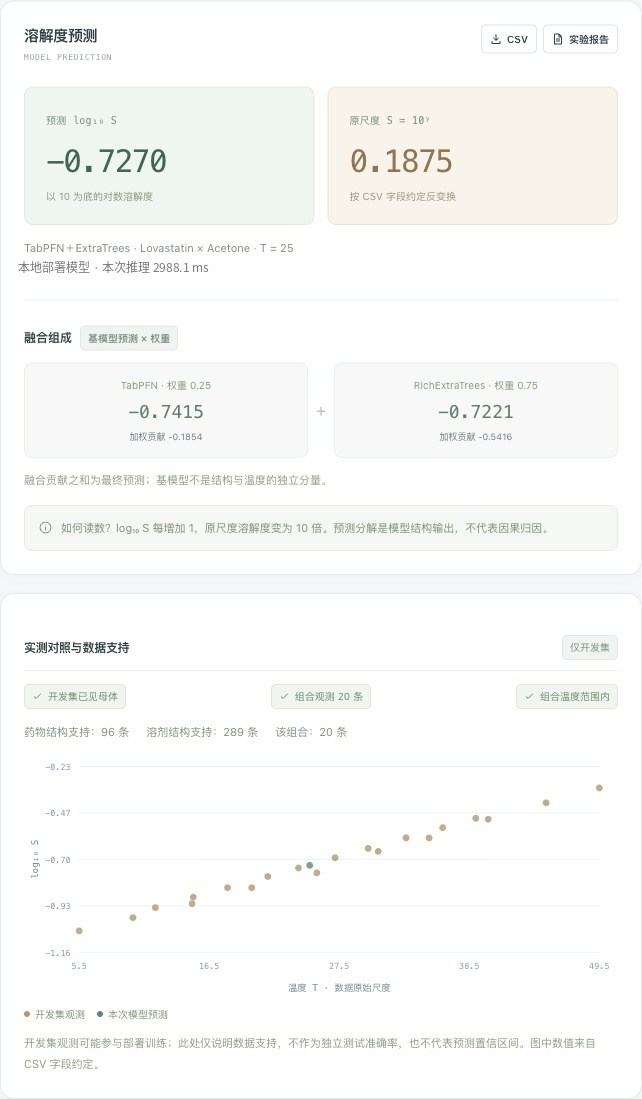
\includegraphics[width=\linewidth,height=0.48\textheight,keepaspectratio]{app_prediction.jpg}
\caption{Screenshot of the single-point conditional-solubility prediction and decision-support interface.}
\label{fig:v2-app-example}
\end{figure}

In the single-point module, users either pick from 186 built-in drugs and 49 common industrial solvents via drop-down menus or type a custom SMILES. For lovastatin in acetone at $25^\circ\text{C}$, the model returns its answer in 1.7 s: a log-solubility of $-0.7270$, i.e.\ $0.1875\ \mathrm{mol/L}$. The interface shows the ExtraTrees branch output ($-0.7270$) alongside the TabPFN contribution, keeping the whole prediction transparent.

To guard against blind extrapolation, the system provides a coverage and applicability-domain indicator. With each prediction it queries the underlying chemical database and displays how many measurements of that combination exist in the training set (lovastatin--acetone has 20 records, spanning $[5.5^\circ\text{C}, 49.5^\circ\text{C}]$). When the queried condition falls outside the supported temperature window, a prominent warning flags the extrapolation risk.

The process-assistance module offers one-click side-by-side comparison of SOLAR-H and ExtraTrees--TabPFN plus a continuous temperature-response scan. Within a user-chosen window the system generates 61 evenly spaced test points, plots the two response curves, and overlays the historical measured points, helping process engineers judge the solubilisation trend and the models' agreement.

For virtual screening, a high-throughput batch CSV engine accepts files of 1--100 candidate conditions. The backend validates formats, computes features, and runs batch inference asynchronously, flagging bad rows (illegal SMILES or non-physical temperatures) and exporting a structured prediction report.

\subsection{System Verification}

To verify reliability, we built an automated test suite for the service (100\% coverage, all 25 cases passing) and cross-checked the online system against the offline models (Table~\ref{tab:v2-app-check}).

\begin{table}[htbp]
\centering\small
\caption{Automated verification and robustness stress tests of the prediction system.}
\label{tab:v2-app-check}
\begin{tabularx}{\linewidth}{@{}lllX@{}}
\toprule
Test & Method & Tolerance & Result \\
\midrule
Single-point vs.\ offline consistency & in-memory HTTP request vs.\ Python offline model & absolute deviation $< 10^{-10}$ & \textbf{deviation 0}, online and offline agree exactly. \\
Scan vs.\ single-point alignment & compare the scan curve at $25^\circ\text{C}$ with the single-point endpoint & absolute deviation $< 10^{-5}$ & \textbf{deviation $4.92\times10^{-7}$}, scan and single point agree to high precision. \\
Batch boundary and fault tolerance & inject legal SMILES mixed with malformed input & must intercept & syntax errors intercepted with precise location; valid rows 100\% predicted. \\
High-concurrency latency & 5 standard single-point requests after warm-up & $< 3.0\mathrm{s}$ & mean latency \textbf{1.70 s} (1.68--1.73 s) under GPU acceleration. \\
\bottomrule
\end{tabularx}
\end{table}

The benchmarks confirm that the system reproduces the offline results to zero numerical error while sustaining high throughput and fault tolerance, making it a dependable, easy-to-use tool for intelligent solubility computation.
